\documentclass[reportComp]{thesis}
\usepackage[cpp,pseudo]{mypackage}

\title{模式识别作业三}
\subtitle{上机练习}
\school{数据科学与计算机学院}
\author{陈鸿峥}
\classname{17大数据与人工智能}
\stunum{17341015}
\headercontext{模式识别作业}
\lstset{language=python}

\begin{document}

\maketitle

\begin{question}[\textsection 2.5 Q1]
下面的几道题可能会用到如下的程序:
\begin{itemize}
	\item [(a)] 写一个程序产生服从$d$维正态分布$N(\vmu,\Sigma)$的随机样本
	\item [(b)] 写一个程序计算一给定正态分布及先验概率$P(\omega_i)$的判别函数(式(49)中所给的形式)。
	\item [(c)] 写一个程序计算任意两个点间的欧式距离。
	\item [(d)] 在给定协方差矩阵$\Sigma$的情况条件下,写一个程序计算任意一点$\vx$到均值$\vmu$间的Mahalanobis距离。
\end{itemize}
\end{question}
\begin{answer}
程序如下,采用Python进行编写,并且利用numpy包进行矩阵运算。
\begin{lstlisting}
import numpy as np

def normal_distribution(mu,sigma,size=10):
	"""
	Generate d-dimensional normal distribution N(mu,Sigma)
	mu: d-dim vector
	Sigma: d*d-dim covariance matrix
	n: number of generated points
	"""
	return np.random.multivariate_normal(mu,sigma,size)

def discriminant(x,mu,sigma,p_omega):
	"""
	g(x) = ln p(x|omega) + ln P(omega)
	"""
	d = mu.size
	return -1/2 * Manhalanobis(x,mu,sigma) - d/2 * np.log(np.pi) - 1/2 * np.log(np.abs(np.linalg.det(sigma))) + np.log(p_omega)

def L2(p1,p2):
	"""
	Euclidean distance (L2 distance)
	"""
	# return np.linalg.norm(p1-p2)
	return np.sqrt(np.sum(np.power(p1-p2,2)))

def Manhalanobis(x,mu,sigma):
	"""
	Given covariance matrix Sigma, compute the Manhalanobis distance
	from point x to mean mu
	"""
	return (x-mu).T.dot(np.linalg.inv(sigma)).dot((x-mu))
\end{lstlisting}

并且编写了一组测试样例进行检验
\begin{lstlisting}
m = np.random.rand(4,10)
mu = np.mean(m,axis=1)
sig = np.cov(m)
v1 = m.T[1]
v2 = m.T[2]
print(normal_distribution(mu,sig))
print(discriminant(v1,mu,sig,1/2))
print(L2(v1,v2))
print(Manhalanobis(v1,mu,sig))
\end{lstlisting}

结果如下图所示。
\begin{figure}[H]
\centering
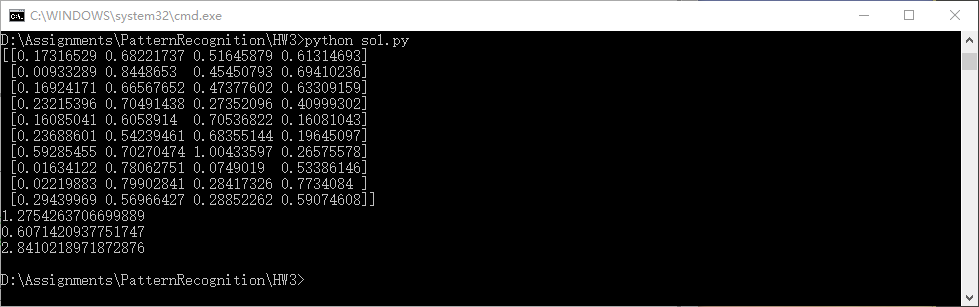
\includegraphics[width=\linewidth]{result.png}
\end{figure}
\end{answer}

\end{document}
% ftp://222.200.180.156/
% student
% 2019s